\documentclass[11pt]{article}
\usepackage[margin=1in]{geometry}
\usepackage{graphicx}
\usepackage{booktabs}
\usepackage{longtable}
\usepackage{array}
\usepackage{caption}
\usepackage{float}
\usepackage{hyperref}
\usepackage{xcolor}
\setlength{\parskip}{0.6em}
\setlength{\parindent}{0pt}

\title{Reddit AI Discourse Analysis Report\\Metaphors, Sentiment, Community Structure, and Engagement}
\author{FrameScope Analysis Pipeline}
\date{May 7, 2026}

\begin{document}
\maketitle

\begin{abstract}
This report summarizes a structured analysis of Reddit discussions about artificial intelligence. The analysis combines metaphor labeling, stance classification, granularity detection, subreddit-level comparison, temporal trend analysis, engagement patterns, and a bubble chart that compares metaphors across communities. The central finding is that Reddit AI discourse is led by practical, tool-oriented language, but that framing coexists with criticism, concern, and a growing move toward discussion of specific models and systems.
\end{abstract}

\section{Executive Summary}
The results point to three broad conclusions.

First, the most common post-level framing treats AI as a useful tool. That does not mean the conversation is cheerful or uncritical. The sentence-level data show that strongly negative framings are also common, especially around ideas such as garbage, criminal behavior, and black-box systems.

Second, framing and sentiment move together. Practical metaphors like tool, assistant, and friend are usually associated with positive language, while metaphors such as weapon, disaster, and black box are more often associated with criticism or concern.

Third, the communities do not all talk about AI in the same way. Some subreddits stay broad and abstract, while others are concrete and model-specific. Over time, the conversation also becomes more specific and more technically grounded. Posts that provoke disagreement tend to draw more comments, even when they do not attract the most agreement.

\section{Methodology}
The analysis is built from sentence-level labels and post-level summaries. Each sentence can carry three major annotation dimensions:
\begin{itemize}
  \item \textbf{Metaphor category}: the dominant figurative frame used to describe AI.
  \item \textbf{Stance}: positive, neutral/unclear, or negative orientation.
  \item \textbf{Granularity}: general AI, model-specific, domain-specific, or not applicable.
\end{itemize}

Sentence-level aggregation captures the language choices used inside individual posts. Post-level aggregation identifies the dominant frame for each Reddit submission. This distinction matters because a single post can contain both praise and criticism, even though engagement is usually recorded at the post level.

The report relies on five figures and two summary tables:
\begin{itemize}
  \item Metaphor--sentiment heatmap.
  \item Community profiles figure.
  \item Temporal metaphor evolution figure.
  \item Engagement matrix.
  \item Subreddit--metaphor bubble chart.
  \item Label distribution table.
  \item Post-dominant metaphor table.
\end{itemize}

\section{Dataset Snapshot}
The summary tables show a consistent pattern. At the post level, the strongest frame is \textbf{Tool}, followed by \textbf{Garbage}, \textbf{Criminal}, \textbf{Assistant}, and \textbf{Black Box}. At the sentence level, \textbf{Tool} again leads by a large margin, followed by the same negative and positive frame families.

Table~\ref{tab:postframes} lists the dominant post-level frames, and Table~\ref{tab:sentenceframes} lists the most common sentence-level combinations.

\begin{table}[H]
\centering
\caption{Top post-level dominant frames}
\label{tab:postframes}
\begin{tabular}{l l l r r}
\toprule
Metaphor & Stance & Granularity & Posts & Pct Posts \\
\midrule
Tool & Positive & Model-Specific & 45281 & 16.63 \\
Garbage & Negative & Model-Specific & 25602 & 9.40 \\
Criminal & Negative & Model-Specific & 22951 & 8.43 \\
Assistant & Positive & Model-Specific & 16809 & 6.17 \\
Black Box & Negative & Model-Specific & 14837 & 5.45 \\
None & Neutral/Unclear & General-AI & 13169 & 4.84 \\
None & Neutral/Unclear & Model-Specific & 11824 & 4.34 \\
Friend & Positive & Model-Specific & 11104 & 4.08 \\
Mind & Positive & Model-Specific & 10373 & 3.81 \\
None & Neutral/Unclear & Not Applicable & 7438 & 2.73 \\
\bottomrule
\end{tabular}
\end{table}

\begin{table}[H]
\centering
\caption{Top sentence-level label combinations}
\label{tab:sentenceframes}
\begin{tabular}{l l l r r}
\toprule
Metaphor & Granularity & Stance & Sentence Rows & Posts \\
\midrule
Tool & Model-Specific & Positive & 77647 & 57370 \\
Garbage & Model-Specific & Negative & 44674 & 34133 \\
Criminal & Model-Specific & Negative & 36881 & 27734 \\
Assistant & Model-Specific & Positive & 28859 & 21467 \\
Black Box & Model-Specific & Negative & 25671 & 19126 \\
None & General-AI & Neutral/Unclear & 22006 & 18535 \\
Mind & Model-Specific & Positive & 20306 & 15864 \\
None & Model-Specific & Neutral/Unclear & 19985 & 17621 \\
Friend & Model-Specific & Positive & 17837 & 14811 \\
None & Not Applicable & Neutral/Unclear & 14099 & 12217 \\
\bottomrule
\end{tabular}
\end{table}

\section{Figure 1: Metaphor and Sentiment}
\begin{figure}[H]
  \centering
  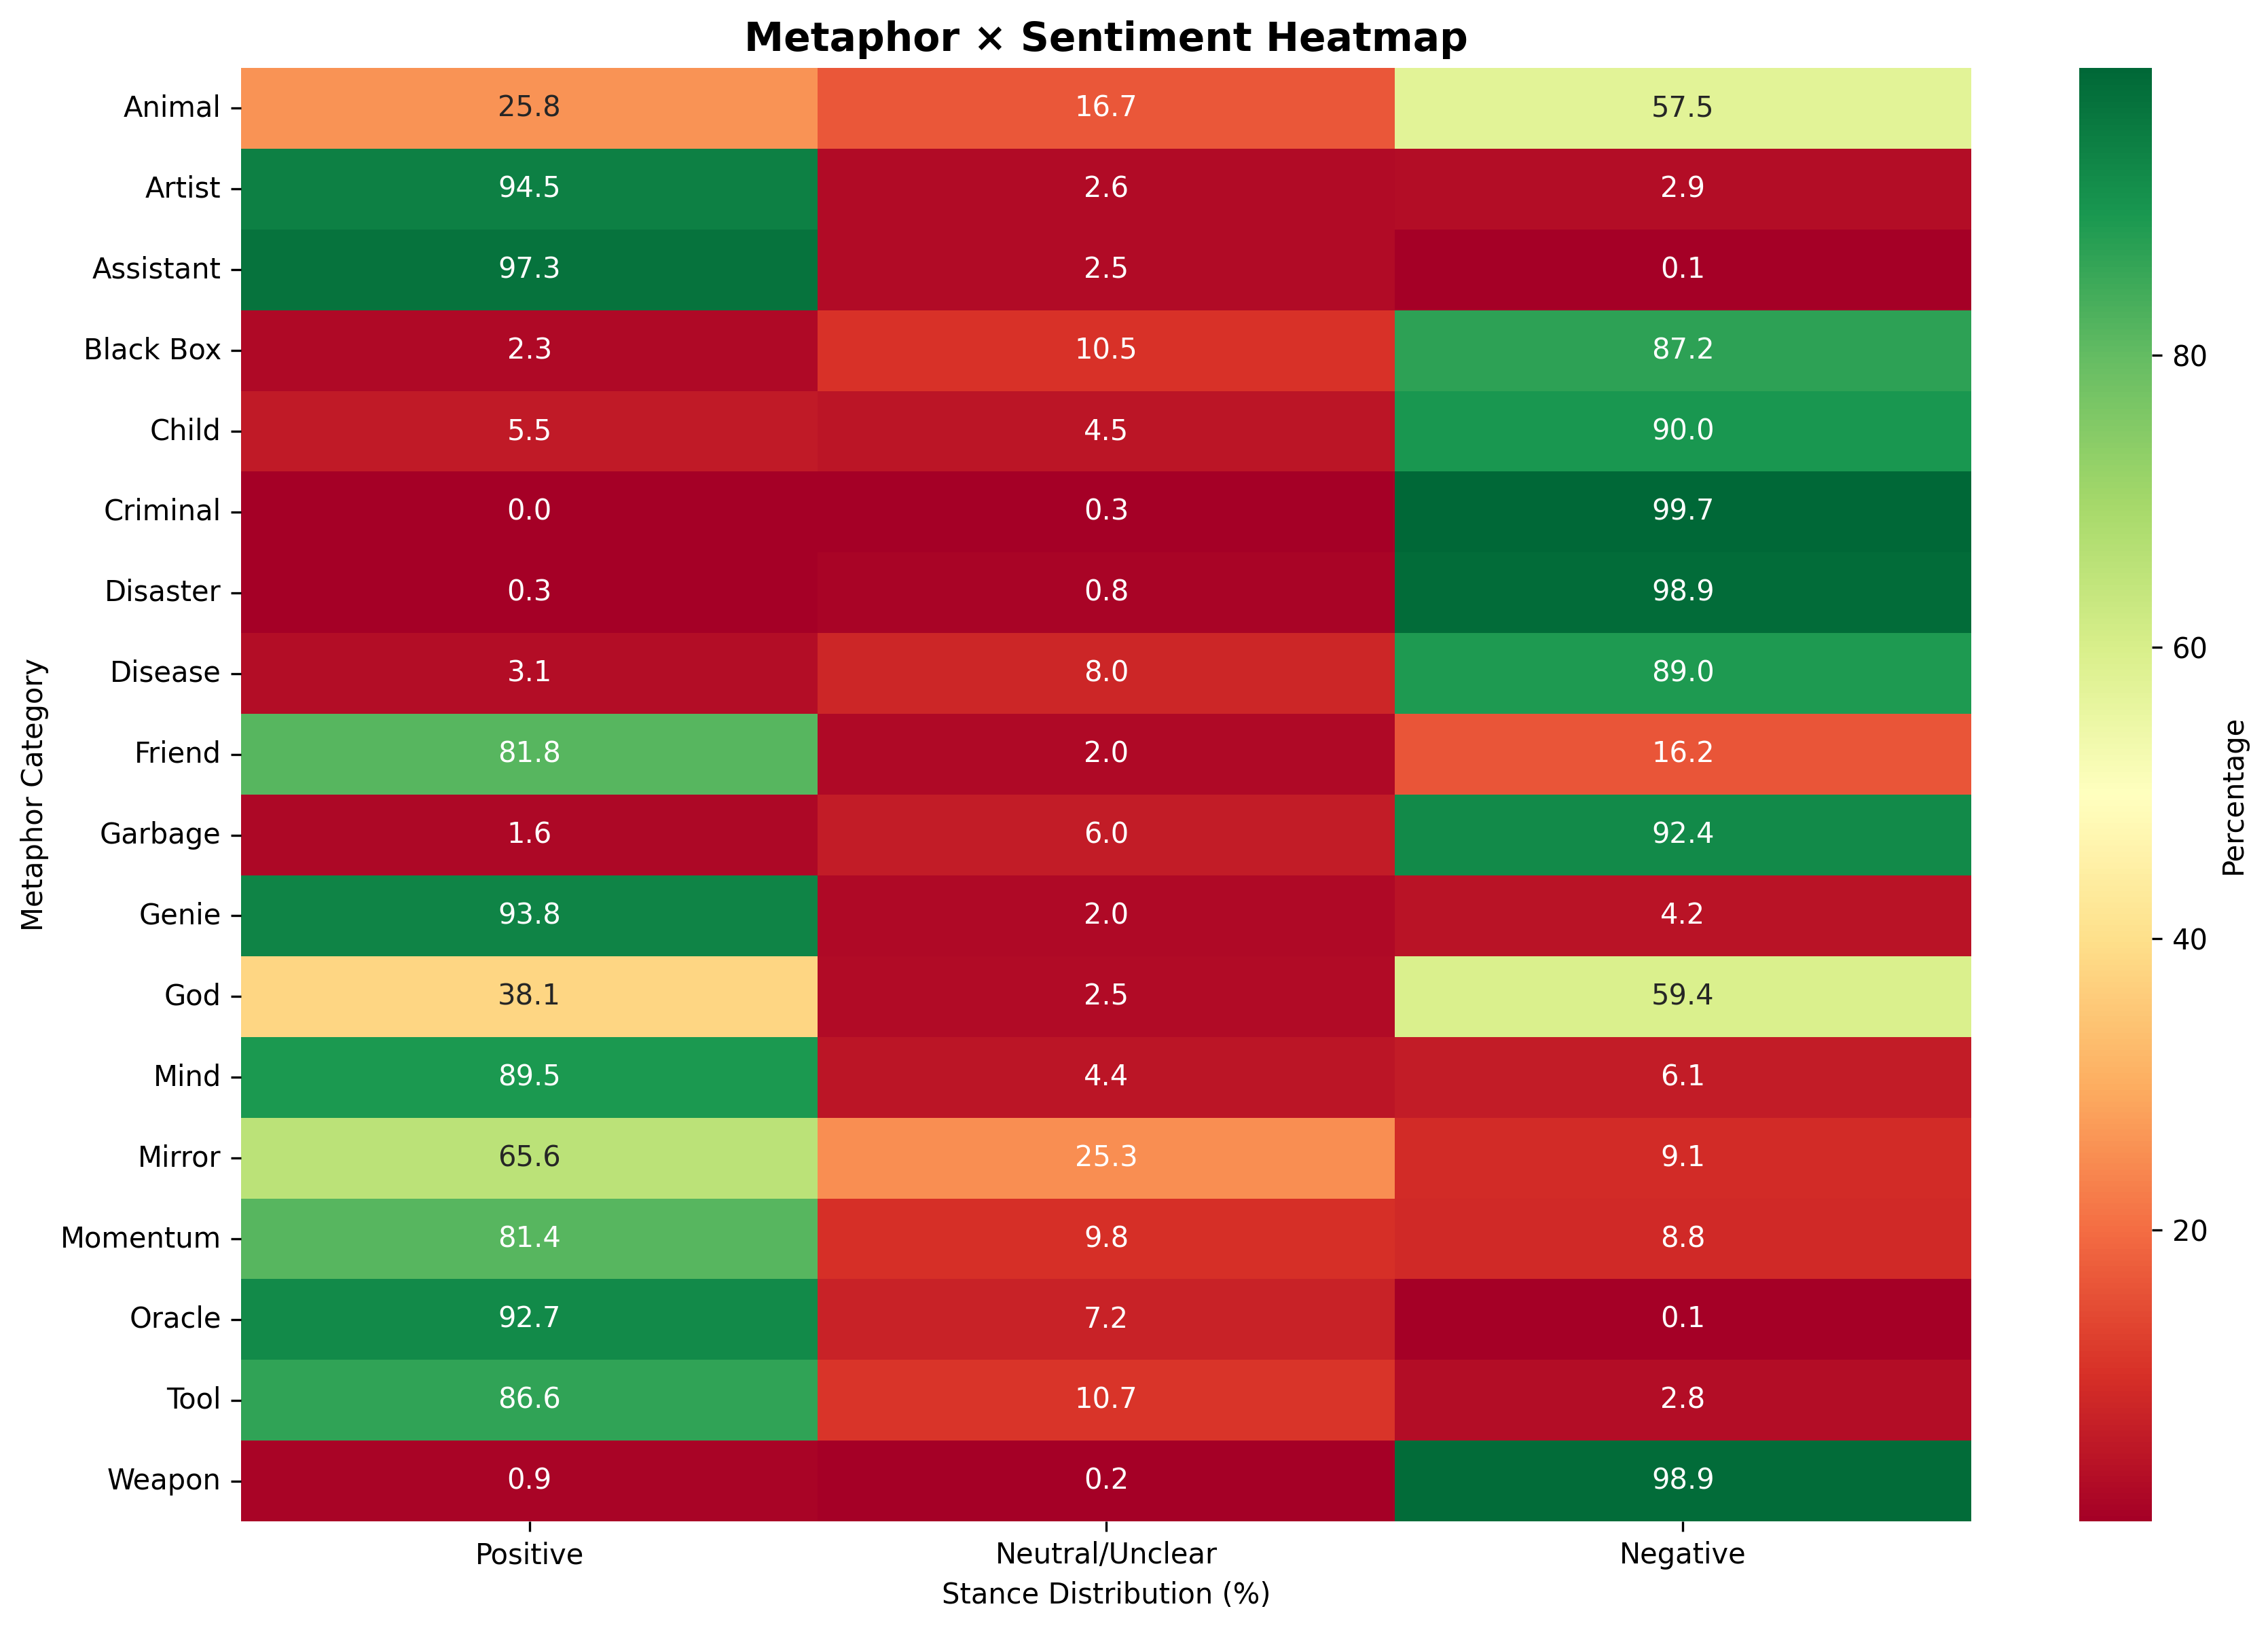
\includegraphics[width=0.95\textwidth]{figures/metaphor_sentiment_heatmap.png}
  \caption{Metaphor--sentiment heatmap showing which frames skew positive, neutral, or negative.}
\end{figure}

The heatmap shows that metaphor choice and sentiment are tightly linked. Tool, assistant, and friend are mainly used in positive settings, while weapon, disaster, garbage, and black box are more often used in negative settings. The ``none'' category remains important because it captures technical language that is not figurative.

The main message is simple: the way people describe AI strongly influences whether the conversation sounds useful, critical, or neutral.

\section{Figure 2: Community Profiles}
\begin{figure}[H]
  \centering
  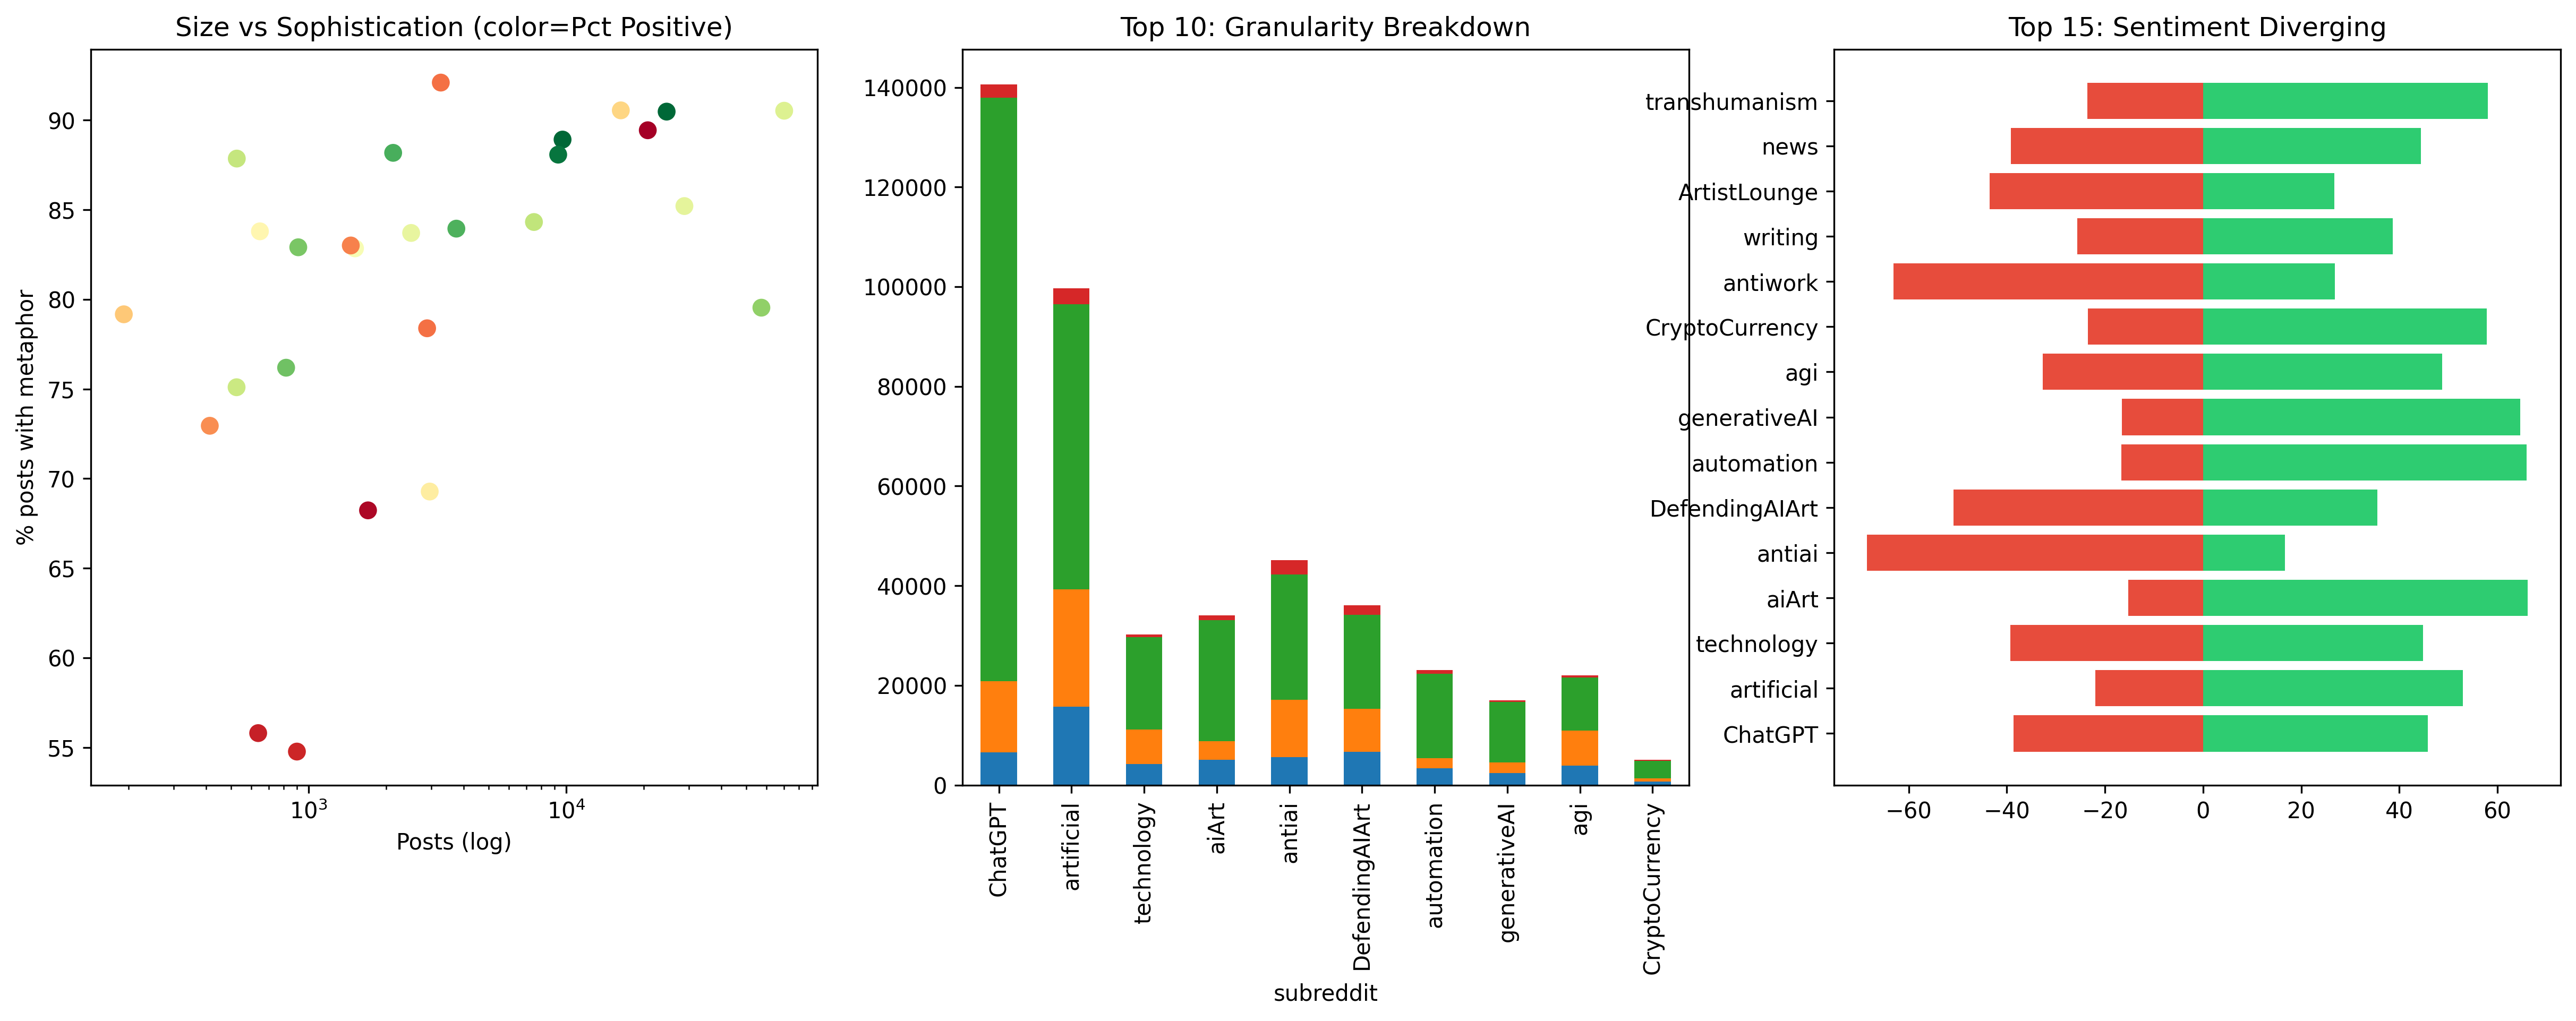
\includegraphics[width=0.95\textwidth]{figures/community_profiles.png}
  \caption{Community profiles combining subreddit size, metaphor usage, granularity, and sentiment balance.}
\end{figure}

The community figure shows that subreddit behavior is uneven. Some communities talk about AI in concrete, model-specific terms, while others stay broad and general. Size does not fully explain this difference.

The scatter panel shows that large communities are not automatically more sophisticated, and small communities are not automatically more abstract. The stacked granularity panel separates broad discussion from specific tool discussion, and the sentiment panel shows that some communities lean practical and positive while others lean cautious or critical.

In practical terms, the figure points to three broad community styles:
\begin{itemize}
  \item \textbf{Practical communities}: tool-focused, optimistic, and specific.
  \item \textbf{Critical communities}: more likely to use negative or risk-oriented frames.
  \item \textbf{Technical communities}: balanced, descriptive, and more likely to mention named systems.
\end{itemize}

\section{Figure 3: Temporal Evolution}
\begin{figure}[H]
  \centering
  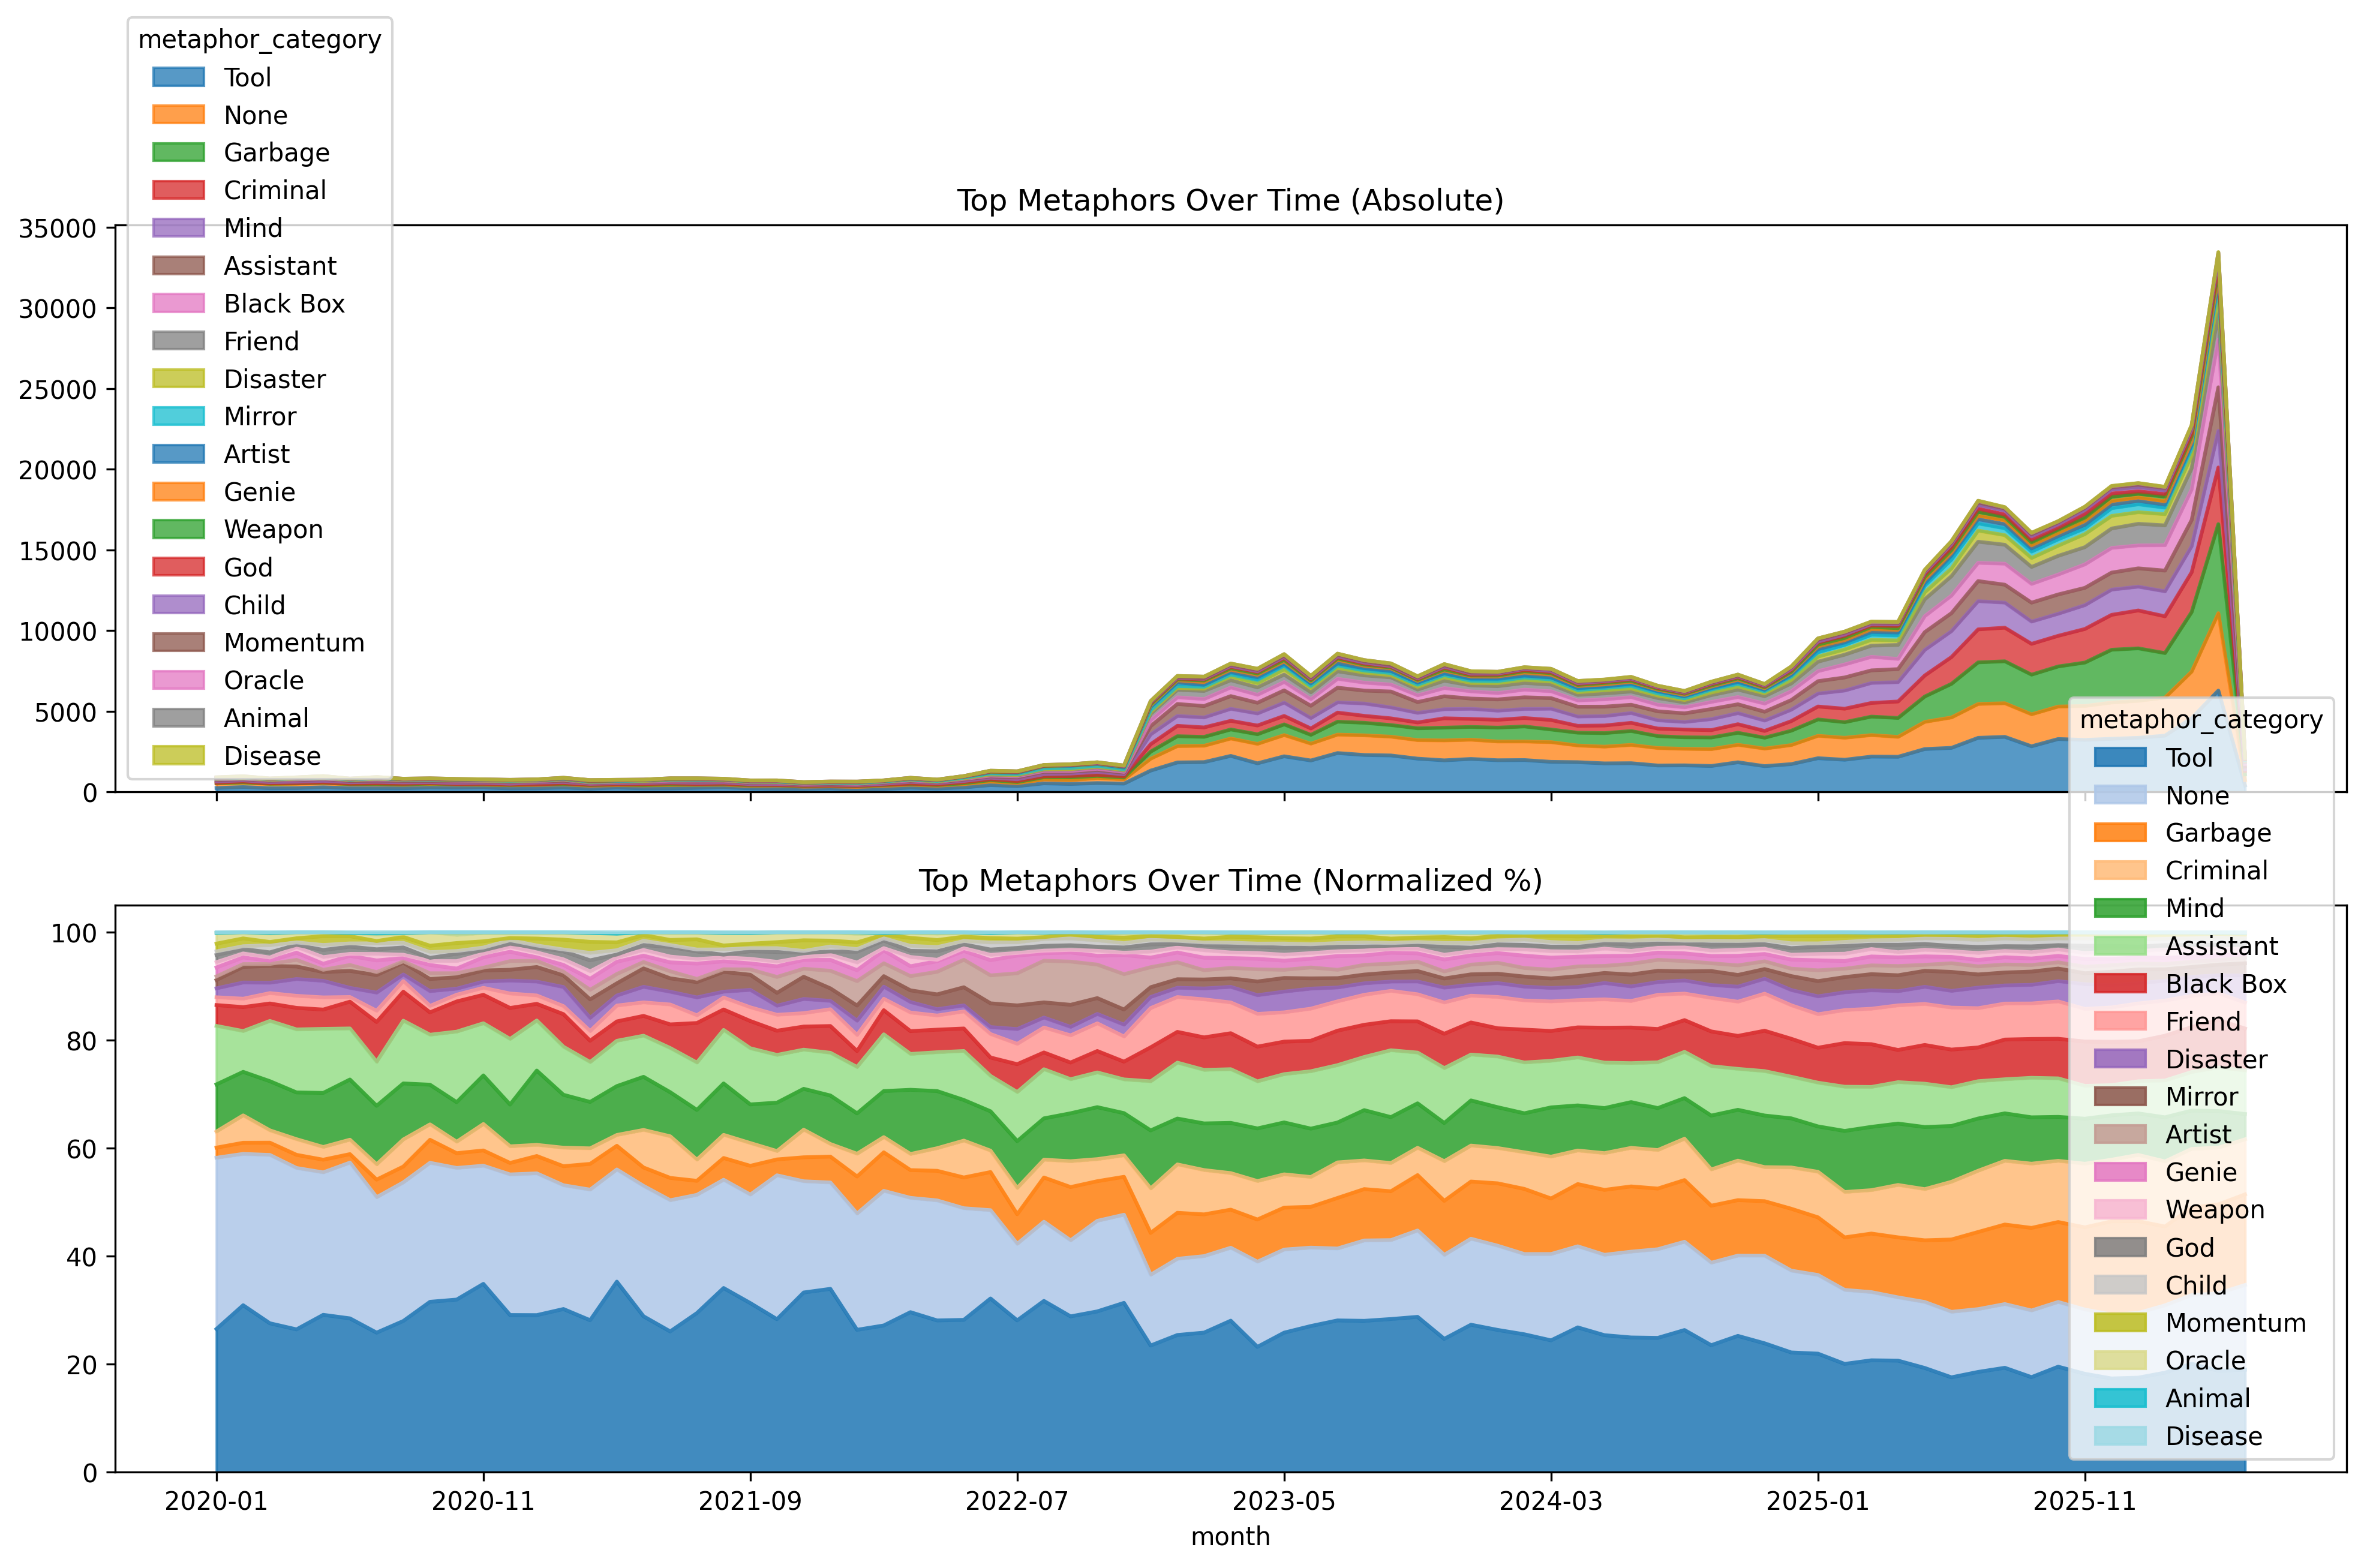
\includegraphics[width=0.95\textwidth]{figures/metaphor_temporal.png}
  \caption{Temporal evolution of the top metaphors in absolute and normalized form.}
\end{figure}

The temporal figure separates volume from composition. The absolute view shows that discussion grows over time. The normalized view shows how the balance of frames changes inside that growth.

The pattern is stable but not static. Tool remains the leading frame, which means usefulness is still the dominant way of talking about AI. At the same time, technical language becomes more prominent, which suggests that the conversation is becoming more concrete and more grounded. Negative frames remain visible as well, which means risk and skepticism grow alongside adoption rather than replacing it.

Overall, the timeline suggests a shift from novelty-driven conversation toward discussion of specific models, specific tools, and specific concerns.

\section{Figure 4: Engagement Matrix}
\begin{figure}[H]
  \centering
  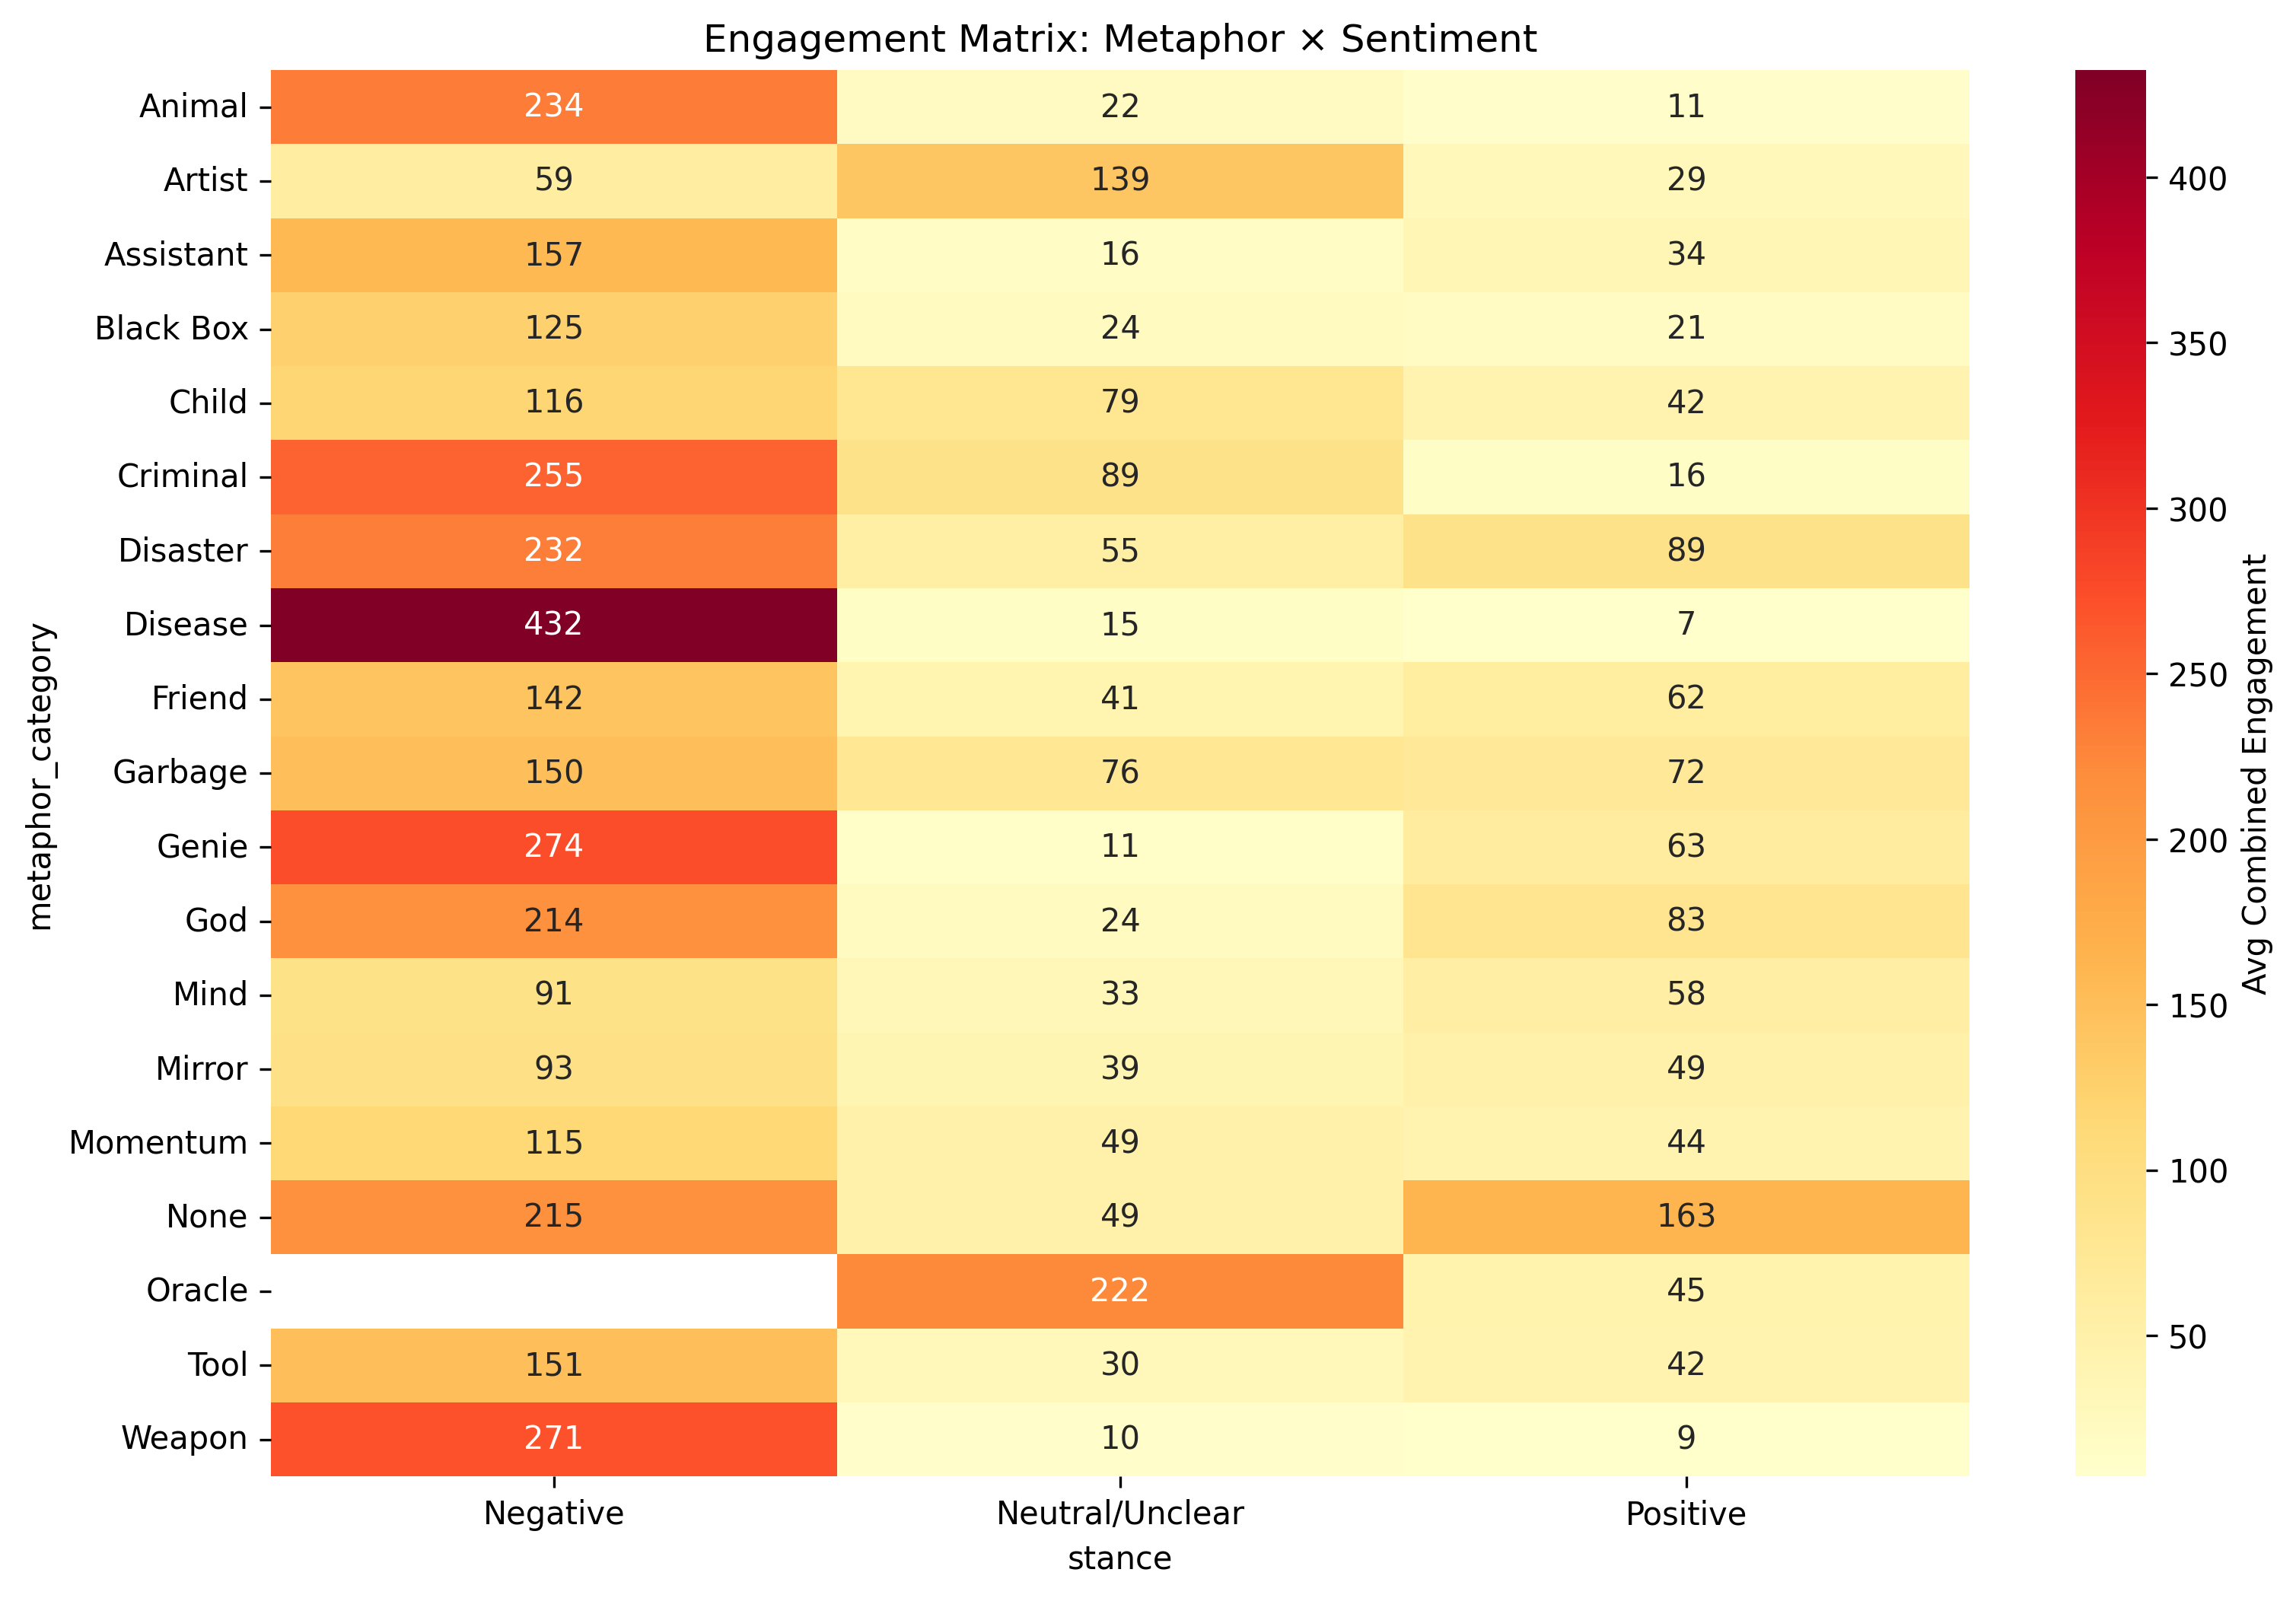
\includegraphics[width=0.95\textwidth]{figures/engagement_matrix.png}
  \caption{Engagement matrix comparing metaphor, stance, and average combined engagement.}
\end{figure}

The engagement matrix separates approval from debate. Positive, practical framing tends to receive more upvotes, while negative or controversial framing tends to attract more comments. That means consensus and discussion are not the same signal.

The main implication is that the strongest frames are not always the most argumentative, but the most argumentative frames often create the most discussion. This means:
\begin{itemize}
  \item \textbf{Tool + Positive} tends to gather broad approval.
  \item \textbf{Weapon + Negative} tends to generate debate or risk discussion.
  \item \textbf{Mind + mixed stance} tends to support philosophical exploration.
\end{itemize}

The matrix shows that sentiment strongly affects audience reaction, but the reaction depends on the frame. Some combinations maximize consensus; others maximize discussion depth.

\section{Figure 5: Subreddit--Metaphor Bubble Chart}
\begin{figure}[H]
  \centering
  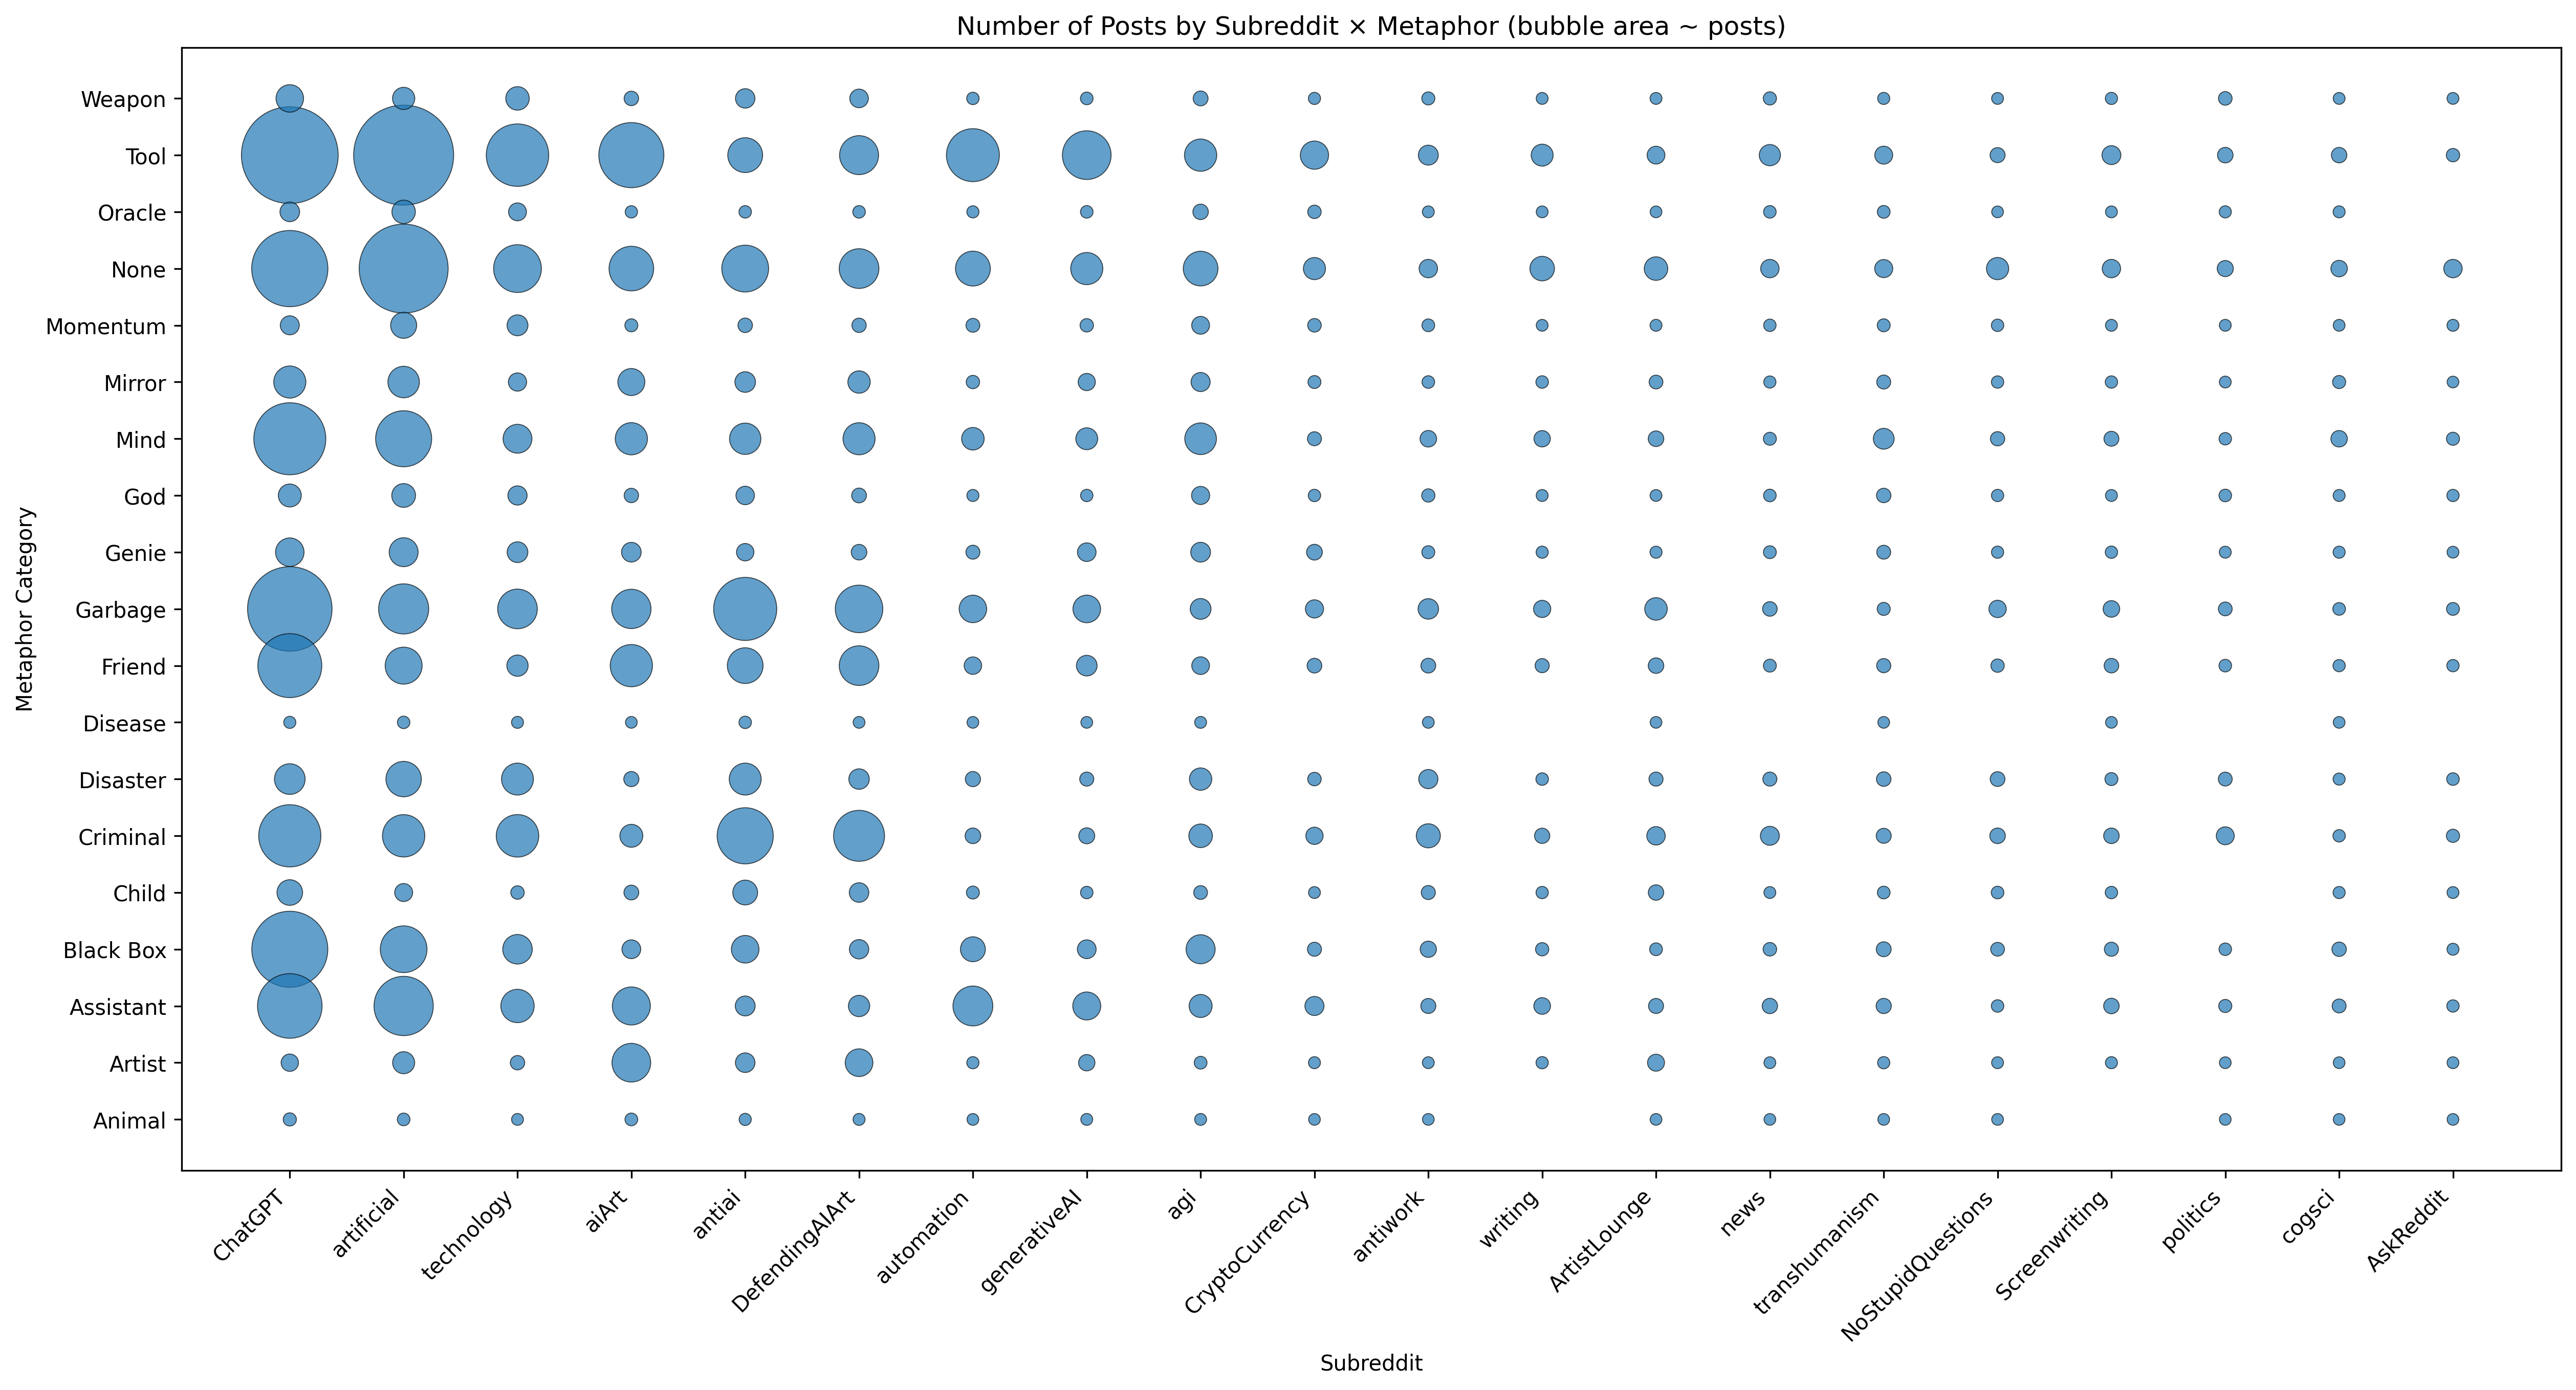
\includegraphics[width=0.95\textwidth]{figures/subreddit_metaphor_bubble.png}
  \caption{Bubble chart of subreddit by metaphor category, where bubble size reflects the number of posts.}
\end{figure}

This figure compares subreddit and metaphor directly. Each bubble shows how often a subreddit uses a particular metaphor, and the bubble area is normalized so the chart stays readable.

The chart is useful because it shows repetition. Large bubbles indicate that a subreddit repeatedly uses the same frame. The vertical position separates practical, critical, and philosophical language. Normalization keeps the biggest communities from overwhelming the display.

Taken together, the bubble chart and the community profile figure show that subreddit identity shapes the language of AI discussion.

\section{Integrated Findings}
Across the figures and tables, the same theme appears repeatedly: Reddit AI discourse is not singular. It is a layered conversation that mixes practical adoption language, technical description, philosophical speculation, and risk framing.

The strongest overall finding is the dominance of \textbf{Tool} framing. At scale, Reddit users often treat AI as something practical to use rather than something purely mysterious or purely threatening. But this practical center does not flatten the discussion. Strong negative frames such as \textbf{Garbage}, \textbf{Criminal}, and \textbf{Black Box} show that criticism is embedded in the conversation.

A second finding is that community identity matters. The same AI topic is discussed differently depending on subreddit norms. Some communities are heavily model-specific, while others stay broad. Some communities are more optimistic, while others emphasize risk. The bubble chart and the community profile figure show that subreddit structure is part of the rhetoric.

A third finding is that the discourse matures over time. The temporal figure shows that broad AI talk does not disappear, but concrete tool-oriented and model-specific discussion becomes increasingly visible. That is what one would expect from a technology moving from novelty to normal use.

\section{Conclusion}
This report shows that Reddit AI discourse is best understood as a dynamic rhetorical ecosystem. The conversation is anchored by practical tool language, tempered by skepticism and risk language, and increasingly organized around concrete systems rather than abstract hype. The figures and tables make that pattern visible across frame distribution, subreddit variation, temporal change, and engagement behavior.

If this report is used for stakeholder communication, the practical takeaway is simple: the words chosen to describe AI shape both sentiment and engagement. If the goal is to explain adoption, use tool-oriented language. If the goal is to surface risk, use critical frames directly. If the goal is to understand public debate, look at community differences rather than averaging them away.

\section{Appendix: Data Files and Reproducibility}
The analysis artifacts are stored alongside this report.
\begin{itemize}
  \item Figures used in the report.
  \item Summary tables used in the report.
  \item The source notebook used to generate the analysis.
\end{itemize}

\end{document}
